\chapter{離散選択モデル}\label{ch:model}
\section{離散選択モデルとは}\label{sec:model_intro}

現実世界では、日々様々な現象が起こっており、その現象の要因もまた複雑に入り組んでいます。こうした膨大な数の現象とその要因を、\textbf{いくつかの仮定の下で整理}し、現象を簡潔な形で表現したもののことを\textbf{モデル}といいます。

\textbf{離散選択モデル}とは、人間の選択行動に関するモデルであって、その選択結果が離散的であるものを指します。

例えば、いくつかある交通手段のうちから一つを選択する交通手段選択行動は、離散選択モデルの枠組みで表現することができます。また、観光客がどの目的地を選んで行くかといった目的地選択行動も、離散選択モデルで表現できます。なお、交通手段選択行動をモデルにしたものを\textbf{手段選択モデル}、目的地選択行動をモデルにしたものを\textbf{目的地選択モデル}等と呼んでいる資料もあります。手段選択モデルや目的地選択モデルは、多くの場合は離散選択モデルとして表現されます。

離散選択モデルを作る目的は、ひとことでいうと、\textbf{ある条件においてどの選択肢がどのくらいの確率で選ばれるのかを推定する}ことです。各選択肢の選択確率が分かれば、現在の総トリップ数に選択確率を掛けることで、乗客数や来訪者数を推定できます。すると、運賃を下げたり所要時間を短縮したりすることが乗客数にどう影響するのか、広場の整備が来訪者数にどう影響するのか、といったことを数値的に示すことができます。

\section{効用最大化の仮定}\label{sec:utility_maxim}

離散選択モデルにおいて一般的に用いられる仮定として、\textbf{「人は効用を最大にする選択肢を選ぶ」という仮定}があります。これはミクロ経済学の最も主要な仮定の一つです。

交通手段選択行動を例にとってみると、人は交通手段を選ぶときに「所要時間」「運賃・駐車場代」「(公共交通機関であれば)頻度」といった様々な要素を天秤にかけて、その中で最終的に一つの交通手段を選んでいます。効用とは、これらの要素を総合的にふまえて決められる単一の数値であり、この効用の値が最も大きくなるような選択肢が常に選ばれる、というのが効用最大化の仮定です。

このように書くと、特定の選択肢に全員が集中してしまうようにも思えますが、そのようなことはありません。

まず、効用の値はその選択肢の性質だけではなく、選択行動をする個人の属性によっても変わるものと考えます。例えば東京から大阪へ行くのに、多くの人は新幹線を使うでしょうが、お金のない学生にとっては運賃が高く感じられ、効用が大きく下がります。逆に夜行バスの効用は、体力や時間的自由がある学生にとってはあまり下がらないかもしれません。

次に、属性が同じであったとしても、最終的な\textbf{効用は確率的に変動する}と考えます。冒頭にも記した通り、モデル化に際しては様々な仮定を置き、現象を簡略化して表現しているので、モデル化に際して考慮されなかった要素を確率的に変化する\textbf{誤差項}としてまとめて考えます。

このような仮定をおくことで、「属性Pの人は選択肢Xを選ぶ傾向にある」といった現象や、「全員がXを選ぶのではなく中には選択肢Yを選ぶ人もいる」といった現象を表現することができます。

\section{確率計算とロジットモデル}\label{sec:mnl}

\subsection{プロビットモデル}\label{ssec:probit}

\ref{sec:utility_maxim}節で述べた通り、効用は確率的に変動するとします。自然な仮定として、効用は正規分布に従うものとすることができます。なお、効用が正規分布に従うとするモデルを\textbf{プロビットモデル}と呼びます。

引き続き、新幹線と夜行バスの例を使うことにします。ある学生Aさんにとって、東京から大阪まで新幹線で移動する場合と夜行バスで移動する場合の効用は図\ref{fig:norm1}のようになりました。

\begin{figure}[ht]
    \centering
    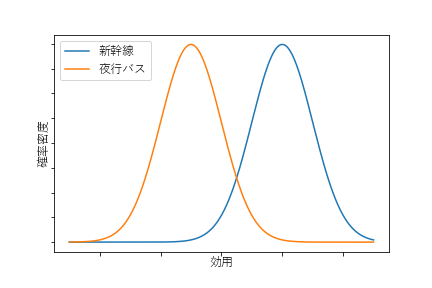
\includegraphics[width=0.5\hsize]{figure/norm1.png}
    \caption{新幹線と夜行バスの効用の比較}
    \label{fig:norm1}
\end{figure}

Aさんにとっては新幹線の方が効用が大きくなる可能性が高く、新幹線が選ばれる確率が高そうです。しかし、必ず新幹線が選ばれるとは限りません。

以下、Aさんにとっての新幹線の効用を $U_S$ 、夜行バスの効用を $U_B$ と書くことにします。$U_S,U_B$ は確率変数になります。ここでは $U_S,U_B$ が\textbf{独立であることを仮定}します。

このとき、Aさんが新幹線を選択する確率は、 $U_S$ が $U_B$ より大きくなる確率であり、 $P(U_S-U_B \geq 0)$ と書くことができます。$U_S$ と $U_B$ が正規分布に従う場合、 $U_S-U_B$ も正規分布に従う\footnote{正規分布の和・差の再生性として知られています。}ため、$P(U_S-U_B \geq 0)$ の値は正規分布の累積確率として求めることができます。

ここに第三の選択肢、飛行機を加えます。この時の効用は図\ref{fig:norm2}のようになります。

\begin{figure}[ht]
    \centering
    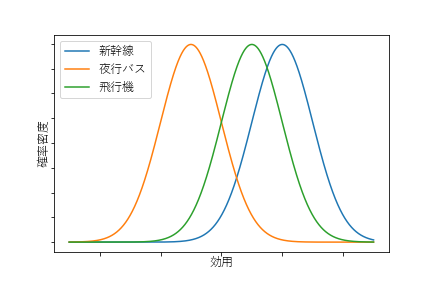
\includegraphics[width=0.5\hsize]{figure/norm2.png}
    \caption{新幹線と夜行バスと飛行機の効用の比較}
    \label{fig:norm2}
\end{figure}


Aさんにとっての飛行機の効用を $U_P$ と書くことにします(当然これも確率変数です)。このとき、この3つの選択肢の中からAさんが新幹線を選択する確率は、 $U_S$ が $U_B$ と $U_P$ より大きくなる確率であり、$P(U_S-U_B \geq 0 \land U_S-U_P \geq 0)$ と書くことができます。また、これを書き換えて $P(U_S - \max(U_B,U_P) \geq 0)$ とすることもできます。

$U_S,U_B,U_P$ が正規分布に従う場合、この確率を計算するのは簡単ではありません。$\max(U_B,U_P)$ が正規分布に従わないため、多重積分によって累積確率を求める必要があるからです。

このように、値を求めるのに積分計算が必要になるような式のことを\textbf{開形式}といい、数値計算上処理が重くなることから嫌われます。先ほどの選択肢が二つしかないバージョンも、正規分布の累積確率を計算するには積分が要るため、開形式です。

選択肢が二つ(二項)の場合であれば、単なる正規分布の累積確率なので数値計算ライブラリを使えば高速に値を求めることができますが、選択肢が三つ以上(多項)で多重積分が必要となると、計算時間が実用上問題になってくる恐れがあります。また数値積分なので誤差の懸念もあります。

そこで、\textbf{正規分布に似た形状の分布を正規分布の代わりに用いる}ことで、積分計算なしで選択確率を計算することが考えられました。

\subsection{ロジットモデル}\label{ssec:logit}

正規分布に形状が似ていて、離散選択モデルの計算上都合がいい性質を持っている分布として、\textbf{ガンベル分布}が用いられます。効用がガンベル分布に従うと仮定したモデルのことを\textbf{ロジットモデル}と呼びます。

ガンベル分布の確率密度関数 $f(x)$ は式(\ref{eq:gumbel_pdf})の通りです。

\begin{equation}
    \label{eq:gumbel_pdf}
    f(x) = \mu \exp(-\mu (x-\eta)) \exp(-\exp(-\mu (x-\eta)))
\end{equation}

また、累積密度関数は式(\ref{eq:gumbel_cdf})の通りです。

\begin{equation}
    \label{eq:gumbel_cdf}
    F(x) = \exp(-\exp(-\mu (x-\eta)))
\end{equation}

ここで、$\mu$ はガンベル分布の\textbf{スケールパラメータ}、$\eta$ は\textbf{ロケーションパラメータ}と呼ばれます。正規分布において平均値 $\mu$ と分散 $\sigma^2$ が与えられれば分布の形状が分かるのと同様に、ガンベル分布においてスケールパラメータとロケーションパラメータが分かれば分布の形状が分かります。

スケールパラメータ $\mu$ は分布のばらつきを意味する値であり、$\mu>0$ でなければいけません。$\mu<0$ だと確率密度関数が負値になってしまいます。

ロケーションパラメータ $\eta$ は分布の最頻値に一致します。

ガンベル分布は、2つの都合の良い性質を示します。

\begin{theorem}
    \label{it:gumbel_max}
    互いに独立な確率変数 $X_1,X_2, \ldots X_i, \ldots, X_N$ が,それぞれガンベル分布\mbox{}\\ $Gb(\eta_1, \mu), Gb(\eta_2, \mu),\ldots,Gb(\eta_i, \mu),\ldots,Gb(\eta_N, \mu)$ に従うとき、$\max(X_1,X_2, \ldots X_i, \ldots, X_N)$ は式(\ref{eq:gumbel_max})に示すパラメータを持つガンベル分布に従う。
    \begin{equation}
        \label{eq:gumbel_max}
        \left(\frac{1}{\mu} \ln\sum_{i=1}^N \exp(\mu\eta_i), \mu\right)
    \end{equation}

    ※ロケーションパラメータは変数ごとに異なっていてもよいですが、\textbf{スケールパラメータは同じ}である必要があります。
\end{theorem}
\begin{proof}
    \ref{prf:gumbel_max}を参照。
\end{proof}

\begin{theorem}
    \label{it:logistic}
    独立な二つの確率変数 $X_1,X_2$ がそれぞれガンベル分布 $Gb(\eta_1, \mu), Gb(\eta_2, \mu)$ に従うとき、その差 $X_1-X_2$ は、式(\ref{eq:logistic})に示す累積分布関数を持つ\textbf{ロジスティック分布}に従う。
    \begin{equation}
        \label{eq:logistic}
        F(x)=\frac{1}{1+\exp(\mu(\eta_1-\eta_2-x))}
    \end{equation}
\end{theorem}
\begin{proof}
    \ref{prf:logistic}を参照。
\end{proof}

この二つの性質を用いることで、積分計算なしに選択確率を計算することができます。

効用 $U_S,U_B,U_P$ が互いに独立でガンベル分布に従うとするとき、新幹線の選択確率 $P(U_S - \max(U_B,U_P) \geq 0)$ を計算します。

まずここで、3つの交通手段の\textbf{効用が従うガンベル分布は、全てスケールパラメータが同一であることを仮定します}。以下、$U_S \sim Gb(V_S, \mu), U_B \sim Gb(V_B, \mu), U_P \sim Gb(V_P, \mu)$ であるとします。

すると定理\ref{it:gumbel_max}により、

\begin{equation}
    \max(U_B,U_P) \sim Gb\left(\frac{1}{\mu} \ln\left(\exp(\mu V_B)+\exp(\mu V_P)\right), \mu\right)
\end{equation}
となります。

ここで $V_S^*=\frac{1}{\mu} \ln\left(\exp(\mu V_B)+\exp(\mu V_P)\right)$ とおき、$U_S=V_S+\varepsilon_S, \max(U_B+U_P)=V_S^*+\varepsilon_S^*$ となるように $\varepsilon_S, \varepsilon_S^*$ を定めると、$\varepsilon_S, \varepsilon_S^*$ はいずれも $Gb(0,\mu)$ に従う確率変数になります。

なお、$V_S$ を\textbf{確定部分}、$\varepsilon_S$ を\textbf{誤差項}と呼ぶことがあります。選択肢の効用 $U$ は確定部分と誤差項の和で表されます。

定理\ref{it:logistic}を用いて、

\begin{equation}
    \begin{aligned}
        P(U_S - \max(U_B,U_P) \geq 0)
         & = P(V_S+\varepsilon_S-V_S^*-\varepsilon_S^* \geq 0)                                                             \\
         & = P(\varepsilon_S^*-\varepsilon_S \leq V_S-V_S^*)                                                               \\
         & = \frac{1}{1+\exp(\mu(V_S^*-V_S))}                                                                              \\
         & = \frac{\exp(\mu V_S)}{\exp(\mu V_S)+\exp(\mu V_S^*)}                                                           \\
         & = \frac{\exp(\mu V_S)}{\exp(\mu V_S)+\exp(\mu \cdot \frac{1}{\mu} \ln\left(\exp(\mu V_B)+\exp(\mu V_P)\right))} \\
         & = \frac{\exp(\mu V_S)}{\exp(\mu V_S)+\exp(\mu V_B)+\exp(\mu V_P)}                                               \\
    \end{aligned}
\end{equation}


より一般に、$N$個の選択肢があって $i$ 番目の選択肢の効用が $Gb(V_i, \mu)$ に従うとき、$j$ 番目の選択肢が選択される確率は、以下の式(\ref{eq:mnl})で表されます。

\begin{equation}
    \label{eq:mnl}
    \frac{\exp(\mu V_j)}{\sum_{i=1}^N \exp(\mu V_i)}
\end{equation}

最後にもう一つ、$\mu=1$ \textbf{であると仮定}すれば、選択確率は以下の式(\ref{eq:mnl_one})で表されます。分子分母を $\mu$ で割ったわけではないことに注意してください。

\begin{equation}
    \label{eq:mnl_one}
    \frac{\exp(V_j)}{\sum_{i=1}^N \exp(V_i)}
\end{equation}

ロジットモデル、特に項が3つ以上の\textbf{多項ロジットモデル(MNL)}では、各選択肢の効用の確定部分 $V_i$ さえわかれば、式(\ref{eq:mnl})や式(\ref{eq:mnl_one})のような平易な式で各選択肢の選択確率を求めることができます。積分が不要な\textbf{閉形式}になっているため、実用上も高速です。

\section{仮定の整理}\label{sec:assumption}

上の選択確率の式(\ref{eq:mnl_one})を導くために、様々な仮定をおいてきました。モデルを実際に適用する際には、これらの仮定がそもそも成り立っているとみなしてよいのか、十分に注意する必要があります。以下、この章でおいた仮定を列挙します。

\begin{enumerate}
    \item 人は効用を最大にする選択肢を選ぶ。
    \item 効用にはランダム性があるが、その分布はガンベル分布に従う。
    \item 各選択肢の効用の分布は互いに独立である。
    \item 効用が従うガンベル分布のスケールパラメータはどの選択肢でも同じである。すなわち、効用のばらつきはどの選択肢でも同じである。
          \begin{itemize}
              \item これは効用の誤差項の分布が全て等しい($Gb(0,\mu)$ に従う)ことを意味する。
              \item 3番目の仮定と合わせて、各選択肢の効用の誤差項は互いに独立かつ同分布であり、このような条件を \textbf{IID} (Independent and Identically Distributed, 独立同分布) と呼ぶ。
          \end{itemize}
    \item スケールパラメータ $\mu=1$ である。
\end{enumerate}

\section{IIA特性}\label{sec:iia}

最後に、ロジットモデルの\textbf{IIA特性}に触れます。

IIA (Independence from Irrelevant Alternatives) 特性とは、二つの選択肢の間の選択確率の比は、その二つの選択肢の効用のみによって決まるという性質のことです。例えばMNLでは二つの選択肢 $i, j$ の間の選択確率の比は $\exp(V_i):\exp(V_j)$ と表されるため、確かにIIA特性を持っているといえます。ロジットモデルのIIA特性は、各選択肢の効用の分布が互いに独立であるという仮定によって生じたものです。

効用の分布が相関するような(似ている)選択肢がある場合、MNLにおける選択確率の計算結果が期待されるものと大きく異なってしまうことがあります。この問題は「\textbf{赤バス青バス問題}」と呼ばれています。

赤バス青バス問題は、次のような問題です。

\begin{itembox}[l]{赤バス青バス問題}
    「車」「赤バス」の二つの選択肢から選ぶロジットモデルにおいて、効用の確定部分が全く同じであれば、両者の選択確率は $1/2, 1/2$ となる。ここに「青バス」という選択肢を加えたとき、これの効用の確定部分も他と同じであったとすれば、三つの選択肢の選択確率は $1/3, 1/3, 1/3$ となる。色違いのバスが登場しただけでもともと車を利用していた人の三分の一もがバスに流れるのはおかしい。
\end{itembox}

赤バス青バス問題は、車と赤バスの選択確率の比が、青バスの有無によらず $1:1$ であるというIIA特性によって生じる問題です。

MNLで選択確率を適切に推定するには、選択肢の中で互いに似ているものがないことが必要です。赤バス青バス問題が起こりそうな場合には、\textbf{Nested Logit モデル}などのより応用的なモデルを用いることになります。
